{
\begin{figure}[hbt]
\newcommand{\figWidtha}{12cm}
\newcommand{\trimfig}[2]{\trimFigb{#1}{#2}{0}{.0}{.1}{.1}}
\begin{center}
 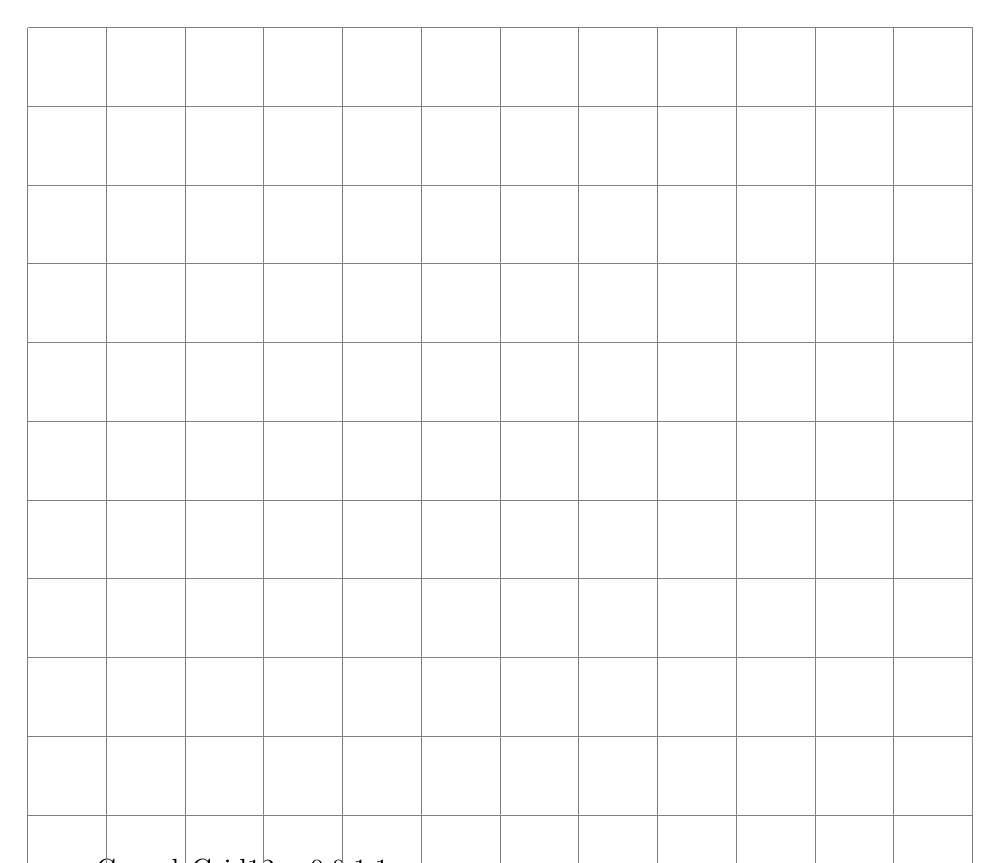
\begin{tikzpicture}[scale=1]
 \useasboundingbox (0,.75) rectangle (12,11);  % set the bounding box (so we have less surrounding white space)
%
 \draw (0,0.0) node[anchor=south west] {\trimfig{marsCapsuleGrid}{\figWidtha}};
%
\draw[step=1cm,gray] (0,0) grid (12,11);
%  \draw (current bounding box.south west) rectangle (current bounding box.north east);
 \end{tikzpicture}
\end{center}
\caption{Space capsule overlapping grid.}
\label{fig:marsCapsule}
\end{figure}
}

%{
%\newcommand{\figWidtha}{12.cm}
%\newcommand{\figWidth}{14.cm}
%\newcommand{\clipfig}[2]{\clipFigb{#1}{#2}{.0}{1.}{.125}{.85}}
%\begin{figure}[hbt]
% \begin{center}
% \begin{pspicture}(0,0)(14,8)
%  \rput(7.,4){\clipfig{marsCapsuleGrid.ps}{\figWidtha}}
% \psgrid[subgriddiv=2]
%\end{pspicture}
%\end{center}
%\caption{Space capsule overlapping grid.}
%\label{fig:marsCapsule}
%\end{figure}
%}
